\chapter*{Introduction (3 pgs)}
\addcontentsline{toc}{chapter}{Introduction}

	The liquid state of $\He$ exists in two phases:
	\begin{itemize}
		\item Helium I - a high temperature phase ($2.17\unit{K}<T<4.2\unit{K}$)
		\item Helium II - a low temperature phase ($T<2.17\unit{K}$)
	\end{itemize}

	These two phases are connected with the \textit{lambda transition}, which occurs at the critical temperature $T_{\lambda} = 2.17 \unit{K}$ at saturated vapour pressure. Helium I is a classical fluid described by ordinary Navier-Stokes (N-S) equations, whereas Helium II indicates the Bose-Einstein condensate (BEC) in much more way.

	\begin{figure}[h]
		\centering
		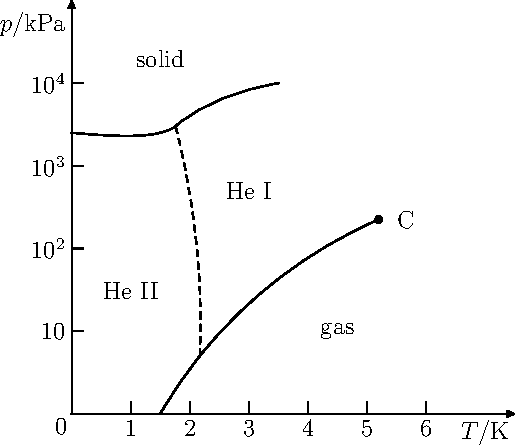
\includegraphics[width=0.5\textwidth]{graphics/theory/phase_diag}
		\caption{Pressure-Temperature diagram of Helium}
		\label{phase}
	\end{figure}

	A simple, phenomenological model of the Helium II motion was proposed by Tisza and Landau - the \textit{two-fluid theory}. Within this model, Helium II is depicted as a mixture of two fluid components, able to penetrate each other:

	\begin{itemize}
		\item normal component - density $\rho_n$, velocity field $\vec{v}_n$, ordinary viscous N-S equation of motion, carrying entropy and thermal excitations represented by \textit{phonons} and \textit{rotons}
		\item superfluid component - density $\rho_s$, velocity field $\vec{v}_s$, modified Euler equation (without viscosity) of motion by quantum terms, no entropy, represented by macroscopic wave function
	\end{itemize}

	The total density of Helium II sums up to $\rho = \rho_n + \rho_s$ and the relative proportion of normal/superfluid component is determined by the temperature. Near $T \rightarrow 0$ Helium II becomes entirely superfluid $\rho_s/\rho \rightarrow 1$. The temperature dependence of this ratio is pretty nonlinear. For example, the ratio $\rho_n/\rho$ drops from $100\%$ at $2.17\unit{K}$ to $50\%$ at $1.95\unit{K}$, to $<5\%$ at $1.3\unit{K}$, and is effectively negligible under $1\unit{K}$.

	\begin{figure}[h]
		\centering
		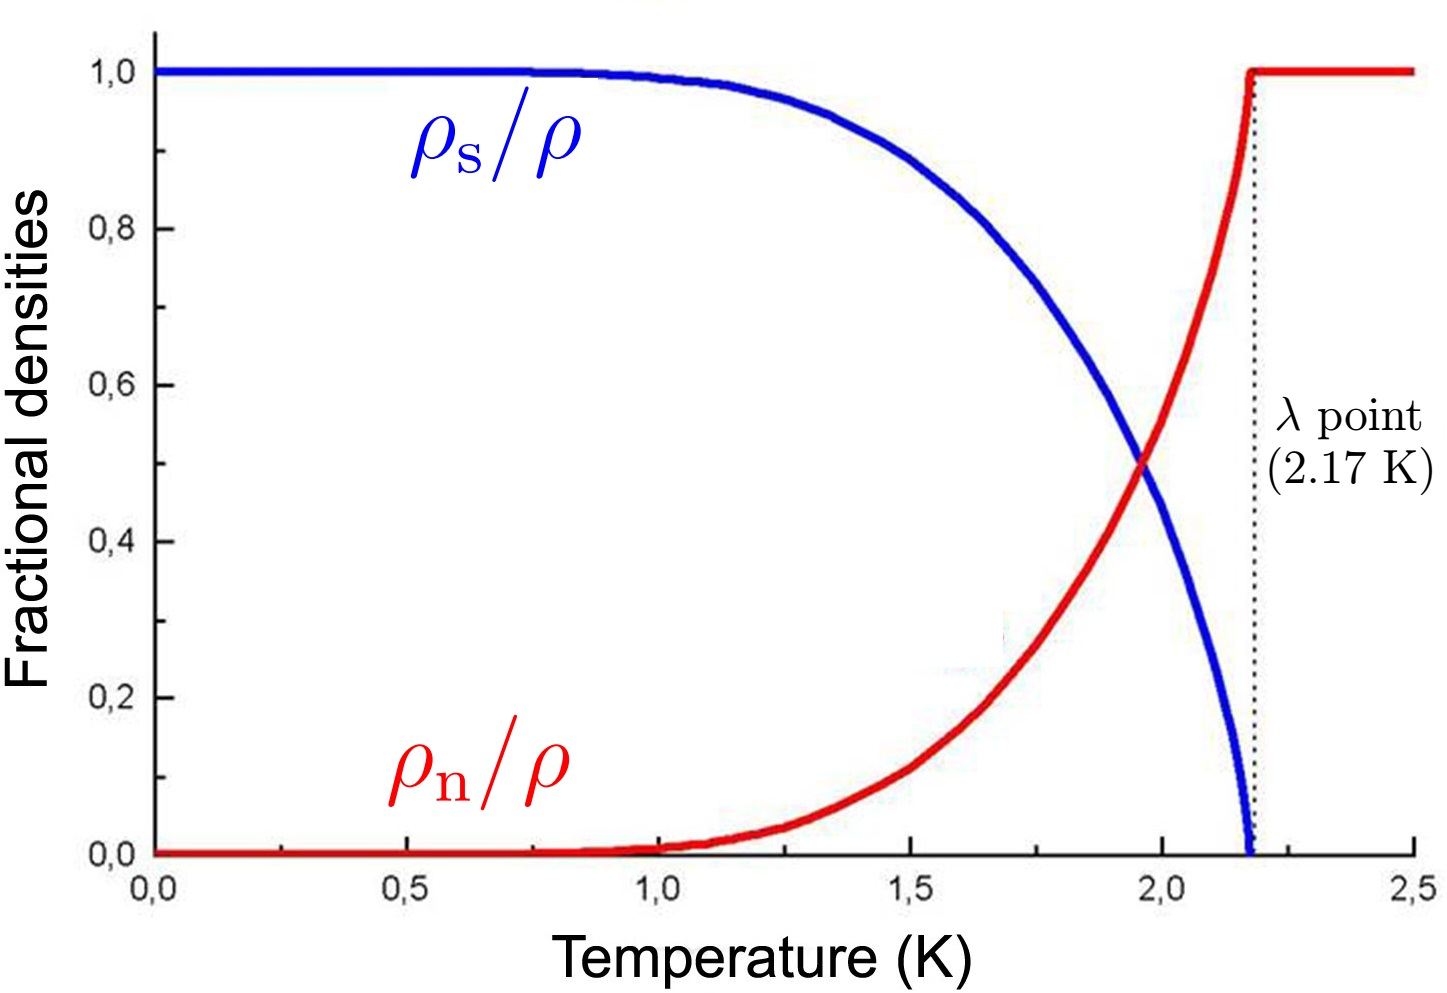
\includegraphics[width=0.7\textwidth]{graphics/theory/densities}
		\caption{Temperature dependence of density proportions}
		\label{densities}
	\end{figure}

	The two-fluid model explains many observed phenomena - among others we pick \textit{second sound} and \textit{thermal counterflow} due to their importance in the study of turbulence.

	\textit{Second sound}: Ordinary sound (the wave of density $\rho$ and pressure $P$) in Helium II is called \textit{first sound}. In such process, temperature $T$ and entropy $S$ is conserved and $\vec{v}_n$ and $\vec{v}_s$ oscillate in phase with each others. On the contrary, a second sound is an antiphase oscillation of $\vec{v}_n$ and $\vec{v}_s$, causing the oscillation of $T$ and $S$ and reamining $\rho$ and $P$ constant. In this work, this phenomena is used for detection of quantized vortices, which naturally appear within Helium II.

	\textit{Thermal counterflow}: Helium II is able to transfer heat in a special way. Let's consider a closed channel filled with Helium II and a dissipating resistor localised at one end of the channel. In normal fluid, the heat is transferred away from the resistor by conduction mechanism. However, in Helium II the heat is carried away only by the normal component. To conserve the total mass flux, some superfluid fluid flow toward the resistor. In this way, a counterflow is generated. If the counterflow is strong enough, the superfluid turbulence is generated.

	It arises from the quantum nature of superfluid, that such fluid cannot perform any rotation. It is called then \textit{irrotational}. However, when Helium II rotates or moves faster than a critical velocity, the circulation is \textit{quantized} and so-called \textit{quantized vortices} are created, which makes the hydrodynamics of Helium II particularly interesting. The vortex nucleation process is still a subject of many current investigations. Superfluid vortex lines can be spatially organized (laminar flows) or completely disorganized (turbulent flows).

	\begin{figure}[h]
		\centering
		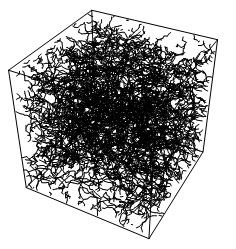
\includegraphics[width=0.4\textwidth]{graphics/theory/QT-tangle}
		\caption{Small simulation cube of tangle of quantum vortices}
		\label{QT}
	\end{figure}

	It has only recently been relized that helium II is an attractive candidate for investigating classical turbulence (CT) problems. Quantum turbulence (QT) can be achieved in many traditional ways - driving a mass flow, spinning discs, oscillating grids and forks, ultrasound, jets. Considering all these methods together, the general trend is that the slow, laminar flow of Helium II (with or without vortices) tends to be rather different from the classical fluid flow. In case of fast motion, the turbulent Helium II seems to behave similar to classical turbulent flow.\\
	To characterize the turbulence we use the dimensionless Reynolds number. Examples of the observed classical features of Helium II QT (regardless on temperature) were found during experiments with flow strength of $\Re \approx 10^6$ (pressure drops), of $\Re \approx 10^5$ (sphere drag crisis), of $\Re \approx 4 \times 10^4$ (whole fluid vorticity) and of $\Re \approx 4 \times 10^3$ (structures of turbulence).

	In classical fluid dynamics (solutions of motion equations), the useful tool for understanding the geometry and dynamics of flow is \textit{vortex filament model}. With the rapid development of available computational power, large simulations have become the methods of choice for calculating the motion of fluids. In superfluids like Helium II, due to the quantization of circulation, vorticity can only exist within vortex filaments with a certain core size, which makes the model a way more applicable than in fields of classical fluids.


	\subsection*{Motivations and Goals}

	Motivations:
	\begin{itemize}
		\item ivestigate transition from CT to QT at various temperatures
		\item prepare clear and reusable codebase for QT simulation
		\item ??
	\end{itemize}

	Goals:
	\begin{itemize}
		\item prepare superfluid Helium II and subsequently generate and detect second sound
		\item generate QT with an oscillating object and measure attenuations
		\item simulate qunatum vortex rings and compare its properties with the theoretical ones
	\end{itemize}

	Motivations: investigate critical velocities and vortex density, create numeric model

	Goals: measure hydrodynamic profiles for more temperatures with oscillating object, transition from CT to QT, investifate numerically vortex rings

\newpage
\chapter{Theoretical Background (15 pgs)}

The theoretical part of this Thesis is composed of two chapters:

\begin{itemize}
	\item[1.] Mesoscopic view - theoretically cover London's theory, creation and numerical modelling of quantum vortex, vortex dynamics.

	\item[3.] Macroscopic view - hydrodynamics of two-fluid model, oscillatory motion in such fluid, creation of QT, existence and usage of second sound

\end{itemize}

The aim of this part of thesis is to introduce the basic properties of quantized vortex lines in Helium II and summarize the main experimental observations of superfluid turbulence. Then there is discussed the theoretical methods used to study quantized vorticity, quantum turbulence and the results obtained using such methods.



\newpage

{\Huge \bfseries Mesoscopic view}
\addcontentsline{toc}{chapter}{Mesoscopic model}
\vspace{0.3cm}

One of the most useful ways of describing superfluid helium at $T=0$ starts with nonlinear Schrodinger equation (NLSE) for the one-particle wave function $\psi$. Since superfluid helium is a strongly correlated system dominated by collective effects, this imperfect Bose condensate is described by Gross-Pitaevskii equation.

\section{Gross Pitaevskii model}

In terms of single-particle wavefunction $\psi(\vec{r},t)$:

\begin{equation}
i \hbar \frac{\partial \psi}{\partial t} = - \frac{\hbar^2}{2m} \nabla^2 \psi
+ \psi \int \vert \psi(\vec{r}^{\prime},t) \vert^2 V(\vert \vec{r} - \vec{r}^{\prime} \vert)
\text{d}\vec{r}^{\prime}\,,
\end{equation}

where $V(\vert \vec{r} - \vec{r}^{\prime} \vert)$ is the potential of two-body interaction between bosons. The normalization is set as $\int \vert \psi \vert^2 \text{d}\vec{r} = N$, where $N$ is number of bosons. By replacing potential with repulsive $\delta$-function of strength $V_0$ one obtains:

\begin{equation}
i \hbar \frac{\partial \Psi}{\partial t} = - \frac{\hbar^2}{2m} \nabla^2 \Psi - m\eps \Psi + V_0 \vert \Psi \vert^2 \Psi\,,
\label{GP}
\end{equation}

where $\eps$ is the energy per unit mass and $\Psi = A e^{i\Phi}$ is a macroscopic wave function of condensate. In this way one can define the condensate's density $\rho_{BEC} = m\Psi\Psi^* =  mA^2$ and velocity $\vec{v}_{BEC} = (\hbar / m)\nabla \Psi$. Note that equation (\ref{GP}) is equivalent to a continuity equation and an modified Euler equation (by the so called quantum pressure term).

Even the superfluid is irrotational $\omega = \nabla \times \vec{v}_{BEC} = \vec{0}$, the NLSE has a vortex-like solution: $\vec{v}_s = \Gamma / 2\pi r\, \vec{e_{\theta}}$, where $\theta$ is the azimuthal angle and $\Gamma=9.97 \times 10^{-4} \unit{cm^2 \dotprod s^{-1}}$ is the \textit{quantum of circulation}, obtained from:

\begin{equation}
\Gamma = \oint_{\mathcal{C}} \vec{v}_{BEC} \cdot \unit{d}\vec{\boldsymbol{\ell}} = \frac{h}{m}
\label{gamma}
\end{equation}

\begin{figure}[h]
	\centering
	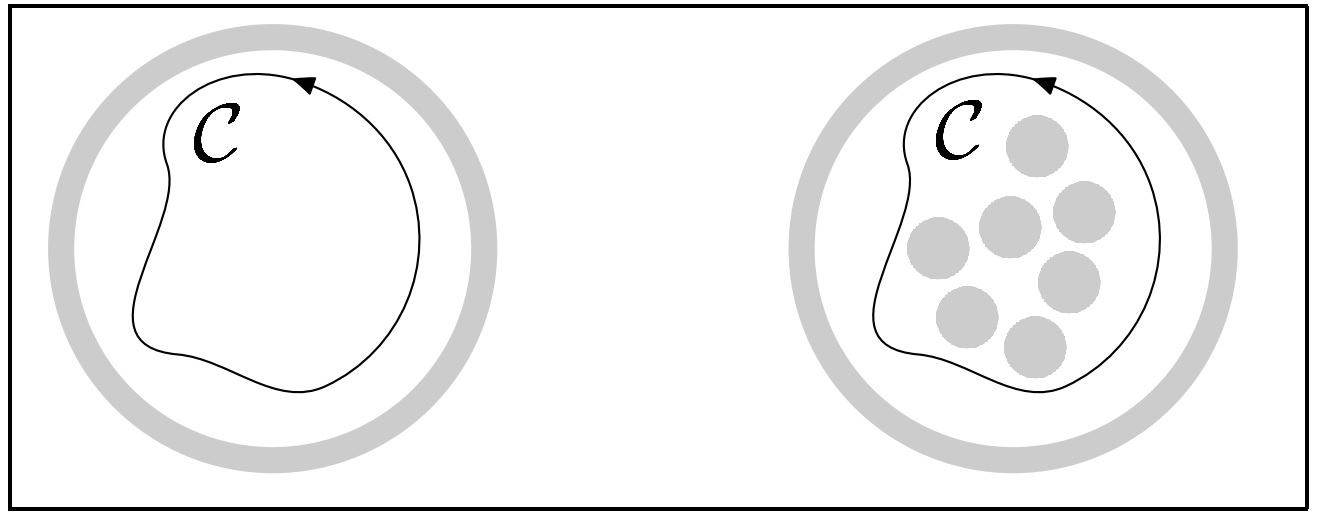
\includegraphics[width=0.5\textwidth]{graphics/theory/singularity}
	\caption{topological singularities within superfluid}
	\label{singularity}
\end{figure}


\section{Quantum vortex}

Superfluid vortex lines appear when helium II moves faster than a critical velocity. Such \textit{nucleation} is the subject of many investigations and is introduced widely later in this work.

The simplest way to create quantum vortices is to rotate cylinder with superfluid Helium II with high enough angular velocity $\Omega$. Created vortex lines form an ordered array of density $L=2\Omega / \Gamma$, all aligned along the axis of rotation. \textit{Vortex line density} $L$ can be also interpreted as a total vortex length in an unit volume.

\begin{figure}[h]
	\centering
	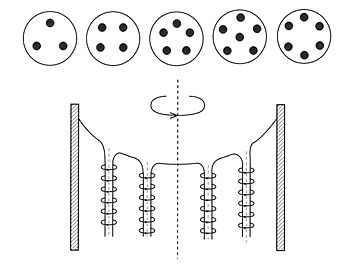
\includegraphics[width=0.4\textwidth]{graphics/theory/rotating-helium}
	\caption{Array of quantized vortices in a rotating container}
	\label{rotating-helium}
\end{figure}

The key properties of Onsager-Feynman vortex are the quantized circulation $\Gamma$, superfluid rotational velocity field $\vec{v}_s = \Gamma / 2\pi r\, \vec{e_{\theta}}$ and the \textit{vortex core parameter} $a_0$. The core size $a_0$ can be estimated by substituting $\vec{v}_s$ back into (\ref{GP}) and solving differential equation for $\rho_s$. One finds that $\rho_s$ tends to the value $m^2 \eps / V_0$ for $r \rightarrow \infty$ and to zero density for $r \rightarrow 0$.
The characteristic distance over which $\Psi$ collapses (superfluid density $\rho_s$ drops from bulk value to zero) is $a_0 \approx 10^{-10} \unit{m} = 1 \unit{\AA}$.

From this, there is a conclusion that the vortex is hollow at its core and therefore, the topological defect occurs. Although, it must be noted that real Helium II is a dense fluid, not weakly interacting Bose gas described by NLSE.

Taking $a_0$ as core radius and $b_0$ as a characteristic distance between two vortices, one can derive the unit length energy for vortex line:

\begin{equation}
\eps_n
= \int_{S_{a_0}}^{S_{b_0}} \eps_{kin}\unit{d}S
= \frac{\pi \hbar^2 \rho_{\ind s} \ln(b_0/a_0)}{m^2}\, n^2
\label{eps_n}
\end{equation}

Since $E_{\ind{vortex}} \sim n^2$, an $N$ quantum vortices contains more energy than $N$ single quantum vortices, and it is generally assumed that only single quantum vortices are commonly observed.

Clearly, vortex lines don't have to be aligned in general. In most cases , the superfluid flow is strongly chaotic, better known as \textit{quantum turbulence}. This topic is covered in more detail later in this work.


\section{Vortex filament model}

The vortex line can be represented as a curve via positional vector $\vec{s} = \vec{s}(\xi, t)$ in three-dimensional space. Here, $\xi$ is arclength along the vortex line. Next we label $\vec{s}^{\prime}$ as $\text{d}\vec{s} / \text{d} \xi$ and $\vec{s}^{\prime\prime}$ as $\text{d}\vec{s}^{\prime} / \text{d} \xi$.
Within our context, $\vec{s}^{\prime}$ is a tangent vector and $\vert \vec{s}^{\prime\prime} \vert$ is a local curvature $R^{-1}$ at a given point. The triad of vectors $\vec{s}$, $\vec{s}^{\prime}$, $\vec{s}^{\prime} \times \vec{s}^{\prime\prime}$ are perpendicular to each other and point along the tangent, normal and binormal respectively:

\begin{figure}[h]
	\centering
	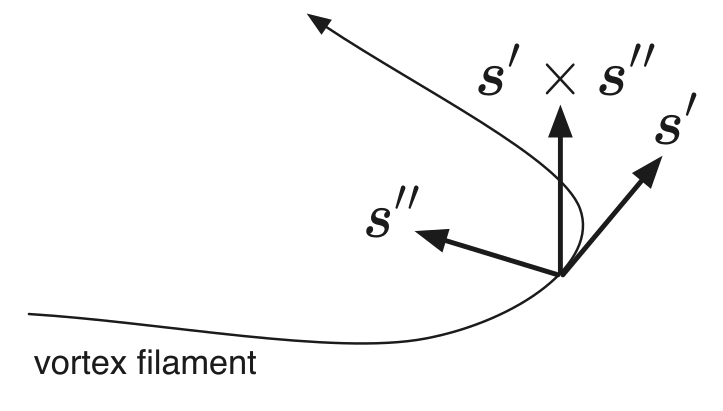
\includegraphics[width=0.5\textwidth]{graphics/theory/filament}
	\caption{Schematic of the vortex filament and the triad vectors}
	\label{filament}
\end{figure}


We suppose that the superfluid component is incompressible $\nabla \dotprod \vec{v}_s = 0$. Moreover, superfluid vorticity $\omega_s$ is localized only at positions of vortex filament $\omega_s(\vec{r},t) = \nabla \times \vec{v}_s$. Combining these two properties gives the Poisson equation $\Delta \phi = \omega_s$ for the potential $\phi$.
Using Fourier transformation one obtains the Biot-Savart law for the superfluid velocity:

\begin{equation}
\vec{v}_s(\vec{r}) = \frac{\Gamma}{4\pi} \int_{\mathcal{L}} \frac{(\vec{r^{\prime}} - \vec{r}) \times \text{d}\vec{r^{\prime}}}{\vert \vec{r^{\prime}} - \vec{r} \vert^3}\,,
\end{equation}

where the integral path $\mathcal{L}$ represents curves along all vortex filaments.

This law determines the superfluid velocity field via the arrangement of the vortex
filaments. Now we define the \textit{self-induced} velocity $\vec{v}_i$, describing the motion which a vortex line induces onto itself due to its own curvature:

\begin{equation}
\vec{v}_i(\vec{s}) = \frac{\Gamma}{4\pi} \int_{\mathcal{L}} \frac{(\vec{r^{\prime}} - \vec{s}) \times \text{d}\vec{r^{\prime}}}{\vert \vec{r^{\prime}} - \vec{s} \vert^3}
\end{equation}

Although, this integral diverges as $\vec{r}^{\prime} \rightarrow \vec{s}$ because the core structure
of the quantized vortex was neglected. We avoid this divergence by splitting the integral into two parts - direct neighborhood of the point $\vec{s}$ (local part) and the rest part $\mathcal{L}^{\prime}$ (nonlocal part). The Taylor expansion of the local part leads to finite result and thus:

\begin{equation}
\vec{v}_i(\vec{s})
= \vec{v}_{\text{s,local}} + \vec{v}_{\text{s,nonlocal}}
\approx \beta \vec{s}^{\prime} \times \vec{s}^{\prime \prime} + \frac{\Gamma}{4\pi} \int_{\mathcal{L}^{\prime}} \frac{(\vec{r^{\prime}} - \vec{s}) \times \text{d}\vec{r^{\prime}}}{\vert \vec{r^{\prime}} - \vec{s} \vert^3}\,,
\end{equation}

where $\beta = (\Gamma / 4\pi) \ln(1/\vert\vec{s}^{\prime}\vert a_0)$. This process is called Local Induction Approximation (LIA). Numerical study of Adachi et al. showed that the nonlocal term plays an important role even for homogeneous quantum turbulence.

Since there could be also external flow source of superfluid component, we define the total superfluid velocity, in laboratory frame, as:

\begin{equation}
\vec{v}_{s,tot} = \vec{v}_{s,ext} + \vec{v}_i
\end{equation}

\section{Vortex dynamics}

To determine the equation of motion of $\vec{s}$ we must recognize the forces acting upon the line - the magnus force $\vec{f}_M$ and (at temperature $T>0$), the drag force $\vec{f}_D$ (both are per unit length).

The magnus force always arises when a rotating body moves in a flow - the rotation creates an increased velocity on one side and decreased velocity on the other one. This causes a pressure difference, which in our case of moving vortex line with circulation quantum $\Gamma$, exerts a force:

\begin{equation}
\vec{f}_M = \rho_s \Gamma \vec{s}^{\prime} \times (\vec{\dot{s}} - \vec{v}_{s,tot})\,,
\end{equation}

where $\vec{dot{s}} = \text{d}\vec{s} / \vec{d} t$ is the velocity of the line filament in the laboratory frame.

The drag force $\vec{f}_D$ arises from the \textit{mutual friction}, the interaction between the normal component and superfluid component. According to Vinen and Hall foundings, the normal fluid flowing with velocity $\vec{v}_n$ past a vortex core exerts a frictional force $\vec{f}_D$ on the superfluid, given by:

\begin{equation}
\vec{f}_D = - \alpha(T)\rho_s\Gamma\vec{s}^{\prime} \times [\vec{s}^{\prime} \times (\vec{v}_n - \vec{v}_{s,tot})] - \alpha^{\prime}(T)\Gamma\vec{s}^{\prime} \times (\vec{v}_n - \vec{v}_{s,tot})
\end{equation}

The temperature dependent dimensionless parameters $\alpha(T)$ and $\alpha^{\prime}(T)$ are written in terms of \textit{mutual friction parameters} $B$ and $B^{\prime}$, which are known from experiments by Samuels and Donnelly:

\begin{equation}
\alpha(T) = \frac{\rho_n B(T)}{2\rho}
\hspace{1cm}
\alpha^{\prime}(T) = \frac{\rho_n B^{\prime}(T)}{2\rho}
\end{equation}

The precise calculation of the mutual friction parameters over the entire temperature range is still an open problem. Although, we already know that friction arises from the scattering process of rotons in the area of high temperatures.

Since the mass of vortex core is usually neglected, the two forces $\vec{f}_M$ and $\vec{f}_D$ sum up into zero: $\vec{f}_M + \vec{f}_D = \vec{0}$. Hence, solving for $\text{d}\vec{s} / \text{d} t$, we obtain the Schwarz's equation:

\begin{equation}
\dot{s} = \vec{v}_s + \vec{v}_i
+ \alpha\vec{s}^{\prime} \times (\vec{v}_{ns} - \vec{v}_i)
- \alpha^{\prime}\vec{s}^{\prime} \times [\vec{s}^{\prime} \times (\vec{v}_{ns} - \vec{v}_i)]\,,
\end{equation}

where $\vec{v}_{ns} = \vec{v}_n - \vec{v}_s$ is the difference between the average velocity of normal fluid and the applied superfluid velocity.

On the basis of Schwarz's equation there can be developed an algorithm to numerically simulate vortex time evolution of an arbitrary configuration. More on this is written later in Simulation part of thesis.

\subsection*{Quantized vortex rings}

A special case of vortex line configuration is a freely moving vortex ring. Such rings are usually created as a result of multi-vortex interconnection and have limited life expectancy. The exact expressions derived by classical hydrodynamics for the energy $E_{\text{ring}}$ and center velocity $v_{\text{ring}}$, moving in a Helium II of density $\rho$ and
having a radius $R$ much greater than its core radius $R >> a_0$, are

\begin{equation}
E_{\text{ring}} = \frac{1}{2}\Gamma^2 \rho R \Big(\ln(8R/a_0) - 2 + c\Big)
\label{ring-energy}
\end{equation}

\begin{equation}
v_{\text{ring}} = \frac{\Gamma}{4\pi R} \Big(\ln(8R/a_0) - 1 + c\Big)\,,
\label{ring-velocity}
\end{equation}

where $c$ is a constant based on inner structure of the vortex. Since we work with hollow core, we use
$c = 0$. Note that (\ref{ring-energy}) and (\ref{ring-velocity}) depend on $a_0$ only logarithmically.
The behavior of the vortex ring is thus quite insensitive to the exact value of $a_0$ (expected to be of the order of atomic dimension).

\todo Life expectancy

\begin{figure}[h]
	\centering
	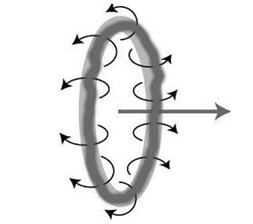
\includegraphics[width=0.3\textwidth]{graphics/theory/vortex-ring}
	\caption{Depiction of quantized vortex ring motion}
	\label{vortex-ring}
\end{figure}

\section{Kelvin waves}

\todo

\newpage

{\Huge \bfseries Macroscopic view}
\addcontentsline{toc}{chapter}{Macroscopic model}
\vspace{0.3cm}

Besides NLSE and Vortex filament model, there is also a third, \textit{macroscopic} model in which the individual vortex lines are invisible. On the other side, Helium II is considered as a continuous flow of vortices.

\begin{figure}[h]
	\centering
	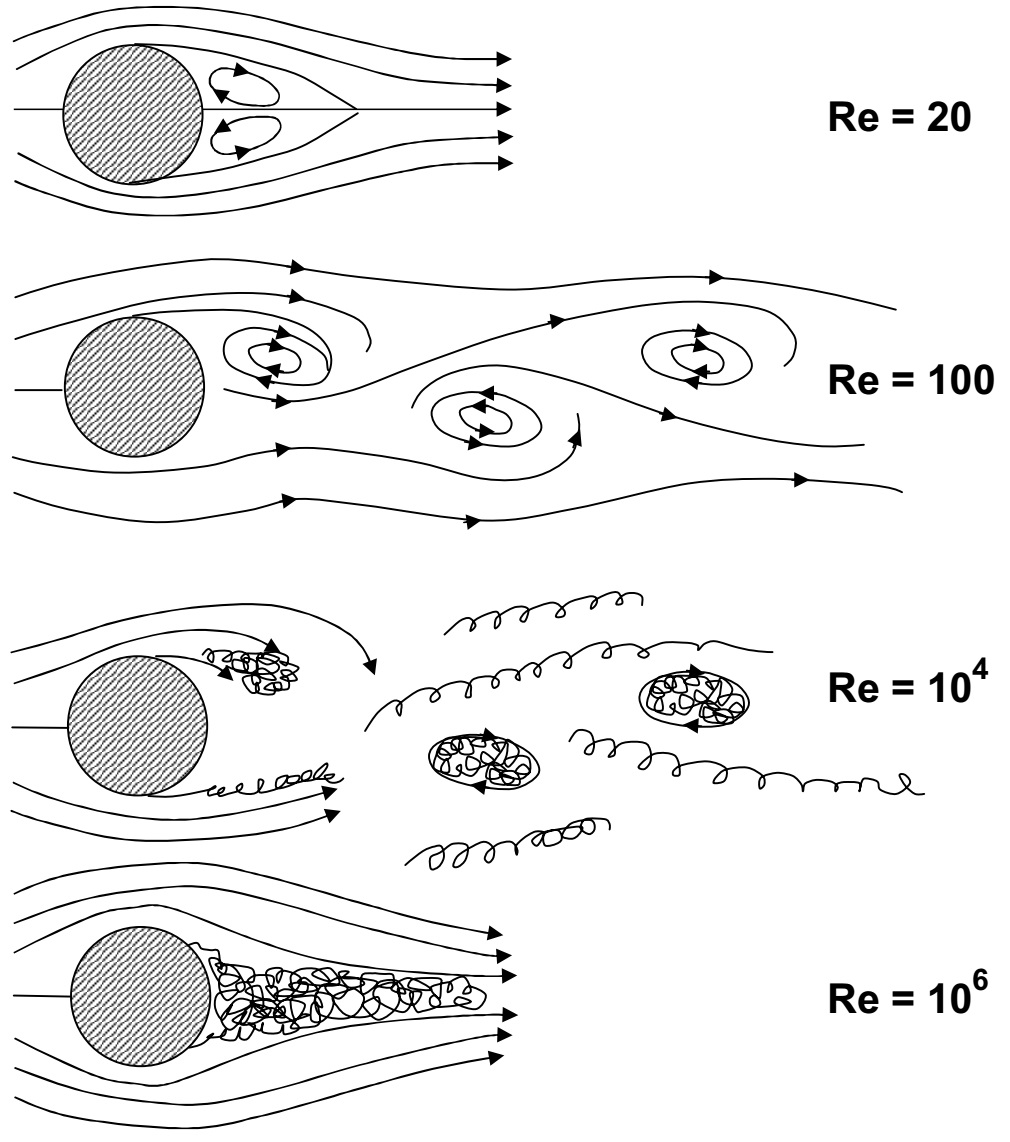
\includegraphics[width=0.5\textwidth]{graphics/theory/laminar-turbulent}
	\caption{transition from laminar to turbulent flow}
	\label{laminar-turbulent}
\end{figure}

\section{Hydrodynamics of superfluid}

Such macroscopic model is called the HVBK model and provides a generalization of Landau's two-fluid model equations, including the presence of vortices. The superfluid is treated as a continuum and we can define a macroscopic superfluid vorticity $\vec{\Omega}_s$, despite the fact that, microscopically, the superfluid velocity field obeys $\nabla \times \vec{v}_s = \vec{0}$. The downside of this model is its assumption of spatially (not randomly) organized vortices. The common example is a rotating cylinder.\\
The incompressible HVBK equations for normal and superfluid component, respectively:

\begin{align}
\frac{\partial\vec{v}_n}{\partial t} + (\vec{v}_n\cdot \nabla)\vec{v}_n =& -\frac{1}{\rho} \nabla P - \frac{\rho_s}{\rho_n} S \nabla T + \nu_n \nabla^2 \vec{v}_n + \vec{F}_{ns}\,,
\label{motion_normal}\\
\frac{\partial\vec{v}_s}{\partial t} + (\vec{v}_s\cdot \nabla)\vec{v}_s =& -\frac{1}{\rho} \nabla P + S \nabla T + \vec{T} - \frac{\rho_n}{\rho} \vec{F}_{ns}\,,
\hspace{15mm}
\label{motion_super}
\end{align}

where we have defined:

\begin{equation}
\vec{\Omega}_s = \nabla \times \vec{v}_s\,,
\end{equation}
\begin{equation}
\vec{F} = \frac{B}{2} \vec{\hat{\Omega}} \times [\vec{\hat{\Omega}}_s \times (\vec{v}_n - \vec{v}_s - \nu_s\nabla \times \vec{\hat{\Omega}})]
+ \frac{B^{\prime}}{2} \vec{\Omega}_s \times (\vec{v}_n - \vec{v}_s - \nu_s\nabla \times \vec{\hat{\Omega}}_s)\,,
\end{equation}
\begin{equation}
\vec{\hat{\Omega}}_s = \vec{\Omega}_s / \vert \vec{\Omega}_s \vert\,,
\end{equation}
\begin{equation}
\vec{T} = -\nu_s \vec{\Omega}_s \times (\nabla \times \vec{\hat{\Omega}}_s)
\end{equation}
\begin{equation}
\nu_s = \frac{\Gamma}{4\pi} \log(b_0 / a_0)
\end{equation}

Here we can identify the quantities as $F$ (mutual friction force), $T$ (tension force) and $\mu_s$ (vortex tension parameter). The intervortex spacing $b_0$ can be estimated as $b_0 = (2\Omega_s \Gamma)^{-1/2}$. Note that two-fluid equations by Landau can be achived by neglecting $\vec{F}$ and $\vec{T}$. The HVBK equations have reasonably set the limits:

\begin{itemize}
	\item $T \rightarrow T_{\lambda}$: In this case $\rho_s \rightarrow 0$ and the normal fluid equation (\ref{motion_normal}) becomes the classical Navier-Stokes equation.
	\item $T \rightarrow 0$: In this case $\rho_n \rightarrow 0$ so the superfluid equation (\ref{motion_super}) describes a pure superflow. Additionally, taking the quantum limit ($\hbar \rightarrow 0$) would take us to the pure Euler equation of viscousless fluid.
\end{itemize}

The HVBK model has been widely used with success to study the transition from classical to quantum turbulence, for estimations of critical Reynolds numbers and its temperature dependence.

\subsection*{Dynamical similarity of flow}

To characterize the turbulence we use the Reynolds number

\begin{equation}
\Re = \frac{UL}{\mu}\,,
\end{equation}

where $L$ is the typical length scale, $U$ the typical velocity scale and $\mu$ the kinematic visocity of the flow field.

In case of stationary $\partial \vec{v} / \partial t = \vec{0}$ fluid mechanics, the principle of \textit{dynamic similarity} is the phenomenon when comparing two geometrically similar vessels (same shape, different sizes) with the same boundary conditions and the same Reynolds numbers, then the fluid flows will be identical. The derivation of this phenomenon can be directly seen from inspection of the underlying motion (\ref{motion_normal}) equation, with geometrically similar bodies. In the classical fluid dynamics of ordinary fluids, we use dynamical similarity and scaling arguments for expressing experimental data in terms of Reynolds numbers, drag coefficients, lift, and so on.

The \textit{drag coefficient} $C_D$ is a dimensionless parameter, representing the relation between \textit{drag force} $\vec{f}$ and fluid velocity $\vec{v}$, and usually takes the form:

$$
C_D \!\propto\! v^\alpha, \hspace{1cm}
\text{where}
\left\{
  \begin{array}{l l}
    \alpha=-1 & \quad \text{for $\Re \in (0-10)$}\\
    \alpha=0 & \quad \text{for $\Re \in (10^3-10^5)$}
  \end{array}
\right.\,.
$$

It is very common to plot experimentally measured dependence $C_D(\Re)$ for various object past flow:

\begin{figure}[h]
	\centering
	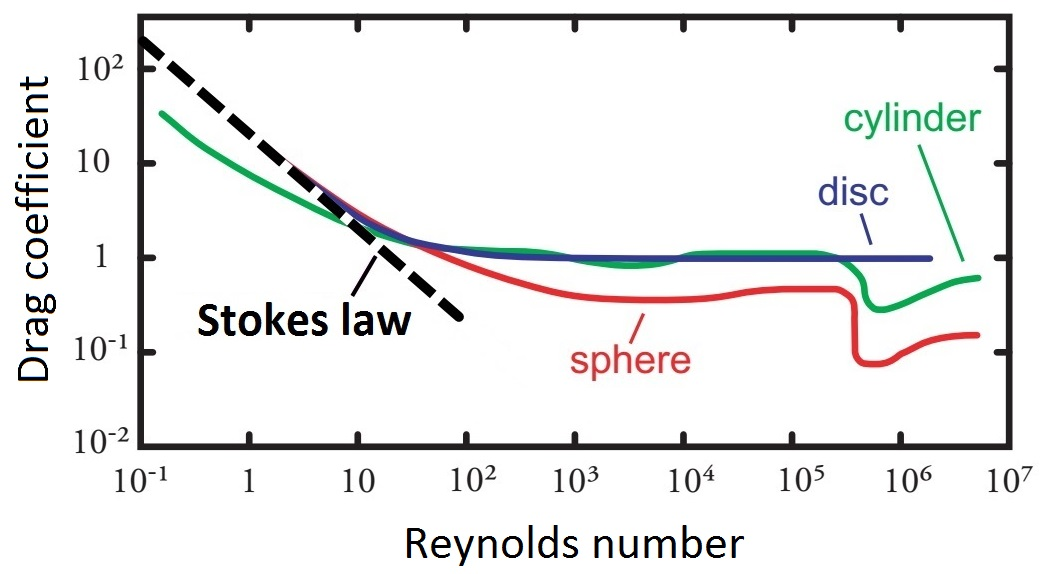
\includegraphics[width=0.7\textwidth]{graphics/theory/C-Re}
	\caption{Drag coefficients of different objects with changing Reynlods number.}
	\label{C-Re}
\end{figure}

Dynamical similarity argument also leads to the existence of critical Reynolds number for normal component, at which the transition to turbulence occurs. For the superfluid component, the Reynolds number can be temperature dependent, which is partial field of investigation of this thesis.


\section{Oscillatory motion in superfluid}

In case of oscillating body in classical viscous fluid, described by ordinary Navier-Stokes equation, the typical length scale $L$, at which the velocity field is changing the most significantly, is identified as the viscous penetration depth:

\begin{equation}
\delta = \sqrt{\frac{2\nu}{\omega}}\,,
\label{penetration}
\end{equation}

where $\omega$ is the angular frequency of oscilations. In the high frequency limit, depending on
body geometry, the substitution $\delta \rightarrow L$ in Reynolds number formula, is correct and
we can calculate an \textit{oscillatory Reynolds number} $\Re_{\delta} = \delta U / \nu$. The reason
for not using the body size is the additional degree of freedom in oscillatory flow (the time
period of one oscillation).

Assuming two independent velocity fields $\vec{v}_n$, $\vec{v}_s$ in Helium II, the above thoughts are applicable for the oscillatory viscous flow of the normal component. We therefore define:

\begin{equation}
\delta_n = \sqrt{\frac{2\nu_n}{\omega}}\,,
\hspace{1cm}
\Re_n = \frac{U \delta_n}{\nu_n}
\label{twofluid}\,,
\end{equation}

The Reynolds number for normal component of Helium II is often called as a \textit{Donnelly number} $D_N$.

In low-frequency mode, when $\delta \ll$ than oscillating body size, the Helium II flow is fully potential and normal component will exhibit a laminar viscous flow. In this case it is shown that the drag coefficient is square-root dependent on oscillation frequency:

\begin{equation}
C_{DN} \propto \sqrt{\nu \omega \propto D_N^{-1}}
\end{equation}

Since the density of normal component is decreasing with temperature, the critical Reynolds number of normal component shifts to higher numbers:

\begin{figure}[h]
	\centering
	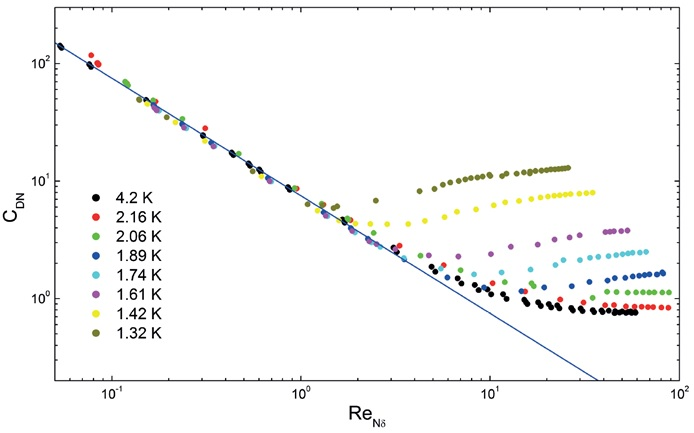
\includegraphics[width=0.8\textwidth]{graphics/theory/C-Re_normal}
	\caption{Drag coefficients vs Reynolds numbers of normal component. The non-constant behaviour of low-temperature curves in turbulent mode are caused due to additional QT.}
	\label{C-Re_normal}
\end{figure}

For the superfluid component, the drag coefficient $C_{DS}$ is defined directly from the hydrodynamic desciption:

\begin{equation}
C_{DS} = \frac{2F_{drag,s}}{A\rho_s U^2}\,,
\end{equation}

where $A$ is a surface, dragged by the flow.

\section{Quantum turbulence}

Superfluid turbulence can be viewed as a tangle of vortex lines and can be generated many ways. The first successful try was done using turbulent thermal counterflow by Vinen. Other popular ways to generate turbulence are

The instability leading to the quantized vorticity is amplified by the self-reconnecting property of vortex loops and the critical velocity $U_{crit}$ is expected to scale with frequency as $U_{crit} \propto \sqrt{\omega}$. Hence we define the dimensionless velocity $\hat{U} = U / \sqrt{\omega}$.\\
A couple of experimental studies in milliKelvin temperatures reported the existence of more critical velocities related with superfluid component flow within single experiment:

\begin{itemize}
	\item \underline{First critical velocity} is related with the formation of quantum vortex rings near the surface of oscillating body - possibly forming a thin layer of different hydrodynamic behaviour. Such critical velocity is hard to observe at higher than ultra-low temperature.

	\item \underline{Second critical velocity} is a consequence of escaping vortex rings from the oscillator body and forming a superfluid bulk or, eventually, the whole turbulent tangle. Here the sudden raise of drag is observed, usually with hysteresis effect.

	\item \underline{Third critical velocity} is the highest critical velocity, which can be observed. The origin of this velocity is hidden in the development of larger quantized vortex structures, which in larger scale become to mimic the classical turbulence. Such velocity is in order $\approx \unit{m/s}$ and therefore, not likely reachable within experiments reported in this thesis.
\end{itemize}

When both velocities of Helium II are high enough, we expect the turbulent regime on both sides to be coupled due to mutual friction and contributing to the drag. In such situation, we are forced to use classical hydrodynamic metrics: drag coefficient $C_D = 2F / (A\rho U^2)$ and Donnelly number $D = U \delta / \nu$. Recent researches also hint that both classical turbulent and quantum turbulent regimes can exist separately with low interaction.

Note that all presented approches are only approximate, since they are neglecting flows near the oscillating body, evaporation processes, sound emissions and other corner-case effects.

\section{Second sound}
\begin{itemize}
	\item attenuation
	\item vortex line density estimate
\end{itemize}

Ordinary sound (the wave of density $\rho$ and pressure $P$) in Helium II is called \textit{first sound}. In such process, temperature $T$ and entropy $S$ is conserved and $\vec{v}_n$ and $\vec{v}_s$ oscillate in phase with each others ($\vec{v}_n(t) \approx \vec{v}_s(t)$). On the contrary, by combination of two-fluid motion and continuity equations, one obtains the wave equation also for the temperature $T$ and entropy $S$. In such case the velocities obey an antiphase oscillation ($\rho_n(t) \vec{v}_n(t) \approx - \rho_s(t) \vec{v}_s(t)$) and remains $\rho$ and $P$ constant.

\begin{figure}[h]
	\centering
	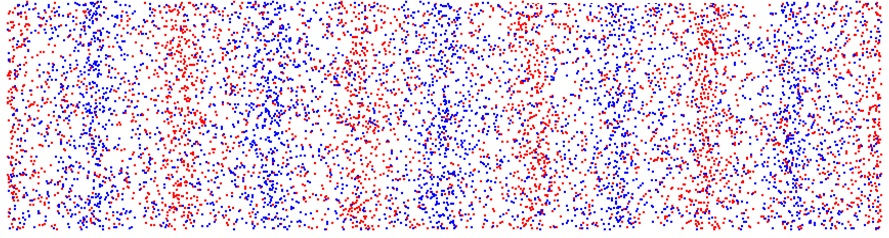
\includegraphics[width=0.99\textwidth]{graphics/theory/ss_1}
	\caption{here will come more proper picture}
	\label{ss_1}
\end{figure}

\begin{figure}[h]
	\centering
	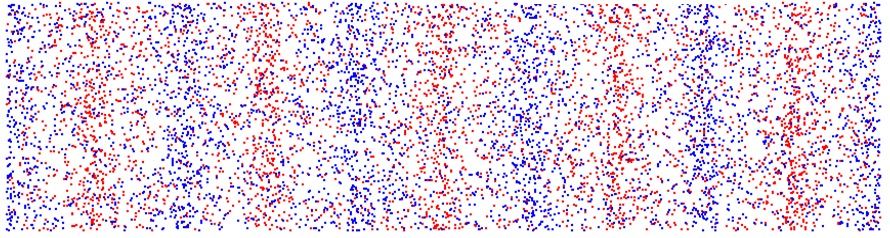
\includegraphics[width=0.99\textwidth]{graphics/theory/ss_2}
	\caption{here will come more proper picture}
	\label{ss_2}
\end{figure}

In early Vinen's observations, the exponentially dumped velocity of second sound wave, propagating through two-fluid medium, was derived from motion equations:

\begin{equation}
\vec{v}_{\ind{ns}} \propto e^{-\alpha \vert \vec{r} \vert} \vec{\hat{e}}_{\vec{r}}(\vec{k},\vec{r},\omega,t)\,,
\end{equation}

where $\alpha$ is the attenuation coefficient. When considering homogeneous chaotic distribution of vortex tangle, one can also derive the formula for the attenuation factor:

\begin{equation}
\alpha = \frac{B\kappa L}{6 \vert \vec{c}_2\vert}
\label{alpha_mean}\,,
\end{equation}

where $B$ is the first mutual friction parameter and $\vec{c_2}$ is the initial second sound velocity. This velocity was experimentally examined and there was found a plateau near the value $20 \unit{m/s}$, which is desirable during experiments (stability against small temperature changes):

\begin{figure}[h]
	\centering
	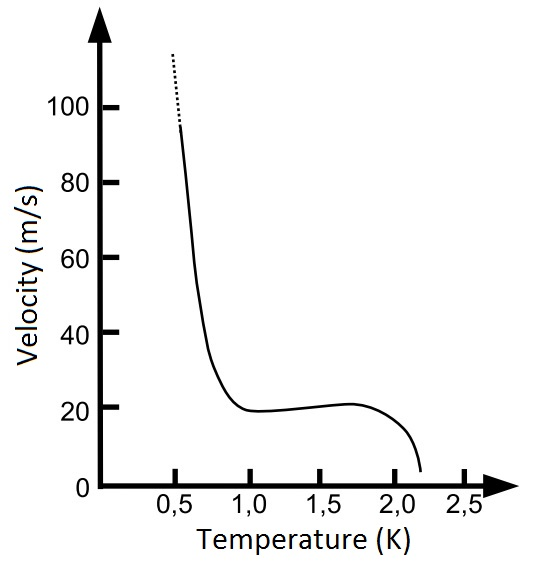
\includegraphics[width=0.4\textwidth]{graphics/theory/ss_velocity}
	\caption{velocity of the second sound with temperature}
	\label{ss_velocity}
\end{figure}

In this work, the phenomenon of second sound attenuation is used for detection of quantized vortices, which naturally appear within Helium II. There is written much more about the method itself within the Experimental Approach part.

\newpage
